It is also important to choose a correct optimizer in order for model to converge as fast as possible. Here 3 different optmizers have been tried out --- SGD, Adam and Adadelta optimizers. As the result SGD optimizer performed the worst, while Adam and Adadelta optimizer performed quite similarly with Adadelta converging to slightly better values at the end. Adam optimizer has required some fine-tuning of the learning rate from 0.001 to 0.0001 to achieve the best result. Both Adadelta and Adam can be used for model optimization in for this dataset. The expreiments were conducted on the truncated dataset of nuclei images using PCC loss.

\begin{figure}[H]
	\begin{center}
		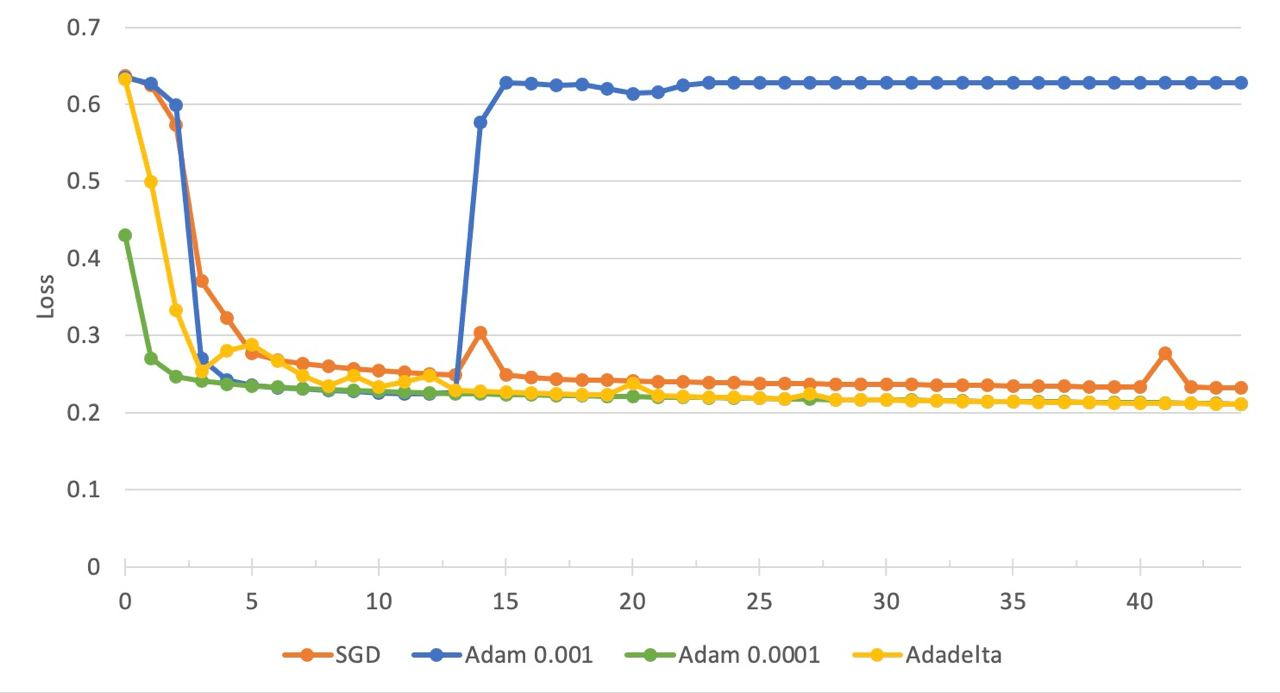
\includegraphics[width=0.8\linewidth]{bilder/model training/optimizer-comparison.jpg}
		\caption{Comparison of convergence for different optimizers}\label{fig:optimizers}
	\end{center}
\end{figure}